\documentclass{article}
\usepackage[italian]{babel}
\usepackage[utf8]{inputenc}
\usepackage[margin=75pt]{geometry}
\usepackage{amsmath}
\usepackage{graphicx}
\usepackage{spverbatim}

%IMPORT CODE
%\usepackage{minted}
\usepackage{listings}
\usepackage{color}

\definecolor{dkgreen}{rgb}{0,0.6,0}
\definecolor{gray}{rgb}{0.5,0.5,0.5}
\definecolor{mauve}{rgb}{0.58,0,0.82}

\lstset{frame=tb,
	language=Haskell,
	aboveskip=3mm,
	belowskip=3mm,
	showstringspaces=false,
	columns=flexible,
	basicstyle={\small\ttfamily},
	numbers=none,
	numberstyle=\tiny\color{gray},
	keywordstyle=\color{blue},
	commentstyle=\color{dkgreen},
	stringstyle=\color{mauve},
	breaklines=true,
	breakatwhitespace=true,
	tabsize=3
}

% in way to comment a block
\long\def\/*#1*/{}

\title{\textbf{Relazione sul Progetto d'Esame}}
\author{Francesco Rombaldoni}
\date{\small Università degli Studi di Urbino Carlo Bo\\
	Insegnamento di Programmazione Logica e Funzionale}

\begin{document}
	\maketitle
	
%	Prepared for a formal document
%	\newpage
	
	%\tableofcontents
	%\newpage

\section{Specifica del Problema}
Scrivere un programma Haskell e un programma Prolog che, dato l'inserimento di due rilevamenti satellitari in formato di coordinata unica nella quale la latitudine e la longitudine sono rappresentate in formato D.M.G internazionale, effettuano le seguenti operazioni: controllo della validità dei rilevamenti inseriti dall'utente, calcolare e riportare (sempre in formato di coordinata unica) per ogni rilevamento la corrispettiva latitudine e longitudine in formato decimale, calcolare e riportare la distanza in chilometri compresa tra i due rilevamenti satellitari, calcolare e riportare l'angolo di rotta espresso in gradi (sia diretto che inverso) che unisce i due rilevamenti inseriti.
\newline
\newline
\emph{[Confrontare lo svolgimento delle fasi successive con quanto riportato nelle prossime pagine.]}\\
\newpage
			
\section{Analisi del Problema}
\subsection{Dati d' Ingresso del Problema}
Per ciascuna delle quattro operazioni, i dati d'ingresso del problema sono rappresentati da due rilevamenti satellitari in formato di coordinata unica nella quale la latitudine e la longitudine sono rappresentate in formato D.M.G internazionale. \\
Esempio di rilevamento accettato: N 40 45 36.000 - E 73 59 2.400.

\subsection{Dati d' Uscita del Problema}
Per ogni inserimento di una coppia di rilevamenti nel formato prima specificato i dati d' uscita del problema, rispettivamente alle ultime tre operazioni descritte all'interno della sezione di specifica del problema, sono: il risultato della conversione delle coordinate del primo rilevamento inserito dal formato D.M.G internazionale a quello decimale, il risultato della conversione delle coordinate del secondo rilevamento inserito dal formato D.M.G internazionale a quello decimale, il risultato del calcolo della distanza compresa tra i due rilevamenti inseriti, il risultato del calcolo dell'angolo di rotta diretto che unisce i due rilevamenti, il risultato del calcolo dell'angolo di rotta inverso che unisce i due rilevamenti. 
L'operazione di controllo della validità dei rilevamenti immessi restituisce un messaggio d'errore nel caso in cui i rilevamenti inseriti non risultino validi. Il messaggio d'errore è composto da due parti, rispettivamente nella prima parte viene descritto il tipo d'errore commesso, mentre nella seconda, viene riportata la porzione di coordinata nella quale è stato rilevato l'errore. 

\subsection{Relazioni Intercorrenti tra i Dati del Problema}
Dato l'inserimento di due rilevamenti nel formato prima specificato, le operazioni in questione sono definite come segue:
\begin{itemize}
	\item Controllo della validità dei rilevamenti; per ogni rilevamento inserito, si verifica che la sua lunghezza sia di trentuno caratteri (considerando anche gli spazi), altrimenti viene restituito un messaggio d'errore. Successivamente si verifica se la latitudine e la longitudine siano corrette, in particolare si verifica se il "segno" della latitudine sia "N" oppure "S", in caso contrario viene restituito un messaggio d'errore, la stessa cosa vale pure per la longitudine, controllando che il "segno" sia "E" oppure "W". Il "corpo" della latitudine e della longitudine si verifica nello stesso modo, controllando se i "gradi" siano compresi tra il valore zero e il valore ottantanove (estremi compresi) e se i "primi" ed i "secondi" siano compresi tra il valore zero ed il valore cinquantanove, qualora i valori dei "gradi", dei "primi" o dei "secondi" dovessero risultare sbagliati, verrà restituito un messaggio d'errore relativo al valore rilevato come errato.
	
	\item Conversione delle coordinate dalla forma D.M.G internazionale alla forma decimale; data una qualsiasi coordinata il passaggio dalla forma D.M.G internazionale alla forma decimale è definito come segue: \\
	Decimali = (Gradi + ( ((Secondi / 60) + Primi) / 60 ) * (-1) se il Segno è  S o W).
	
	\item Calcolo della distanza compresa tra i due rilevamenti inseriti;  data una coppia di rilevamenti rispettivamente denominati "A" e "B" la distanza compresa è definita come: \\
	$Distanza(A, B) = R * \arccos(\sin(latA * \pi / 180) * \sin(latB * \pi / 180) + \cos(latA * \pi / 180) * \cos(latB * \pi / 180) * \cos((lonA - lonB) * \pi / 180)). $\\
	dove R rappresenta il raggio della Terra.
	
	\item Calcolo dell'angolo di rotta diretto e inverso tra i due rilevamenti inseriti; data una coppia di rilevamenti rispettivamente denominati "A" e "B" e data la condizione che la latitudine e la longitudine siano diverse l'angolo di rotta diretto e inverso compresa è definita come: \\
	$\Delta\Phi = \ln( \tan(latB * \pi / 360 + \pi / 4 ) / \tan(latA * \pi / 360 + \pi / 4 )). $\\
	$ \Delta Lon = abs(lonA - lonB). $ \\
	$ Angolo Diretto = atan2((\Delta Lon * \pi / 180), (abs(\Delta\Phi))) / \pi * 180.$\\
	$ Angolo Inverso = Angolo Diretto+ 180.$\\
	Nel caso in cui la latitudini dei due rilevamenti siano identiche:\\
	$\Delta\Phi = \pi / 180 * 0.000000001.$\\
	Nel caso in cui la longitudini dei due rilevamenti siano identiche:\\
	$\Delta Lon = \pi / 180 * 0.000000001.$\\
\end{itemize}
\newpage

\section{Progettazione dell'Algoritmo}
\subsection{Scelte di Progetto}
Il rilevamento immesso dall'utente (nel quale è presente una coppia di coordinate), viene catturato dal terminale sotto forma di "stringa", per tanto, il rilevamento è gestibile come una lista di caratteri "char". Per estrarre le coordinate vengono effettuate delle operazioni arbitrarie volte ad isolare le varie parti della lista d'interesse, proprio per il fatto che queste operazioni sono arbitrarie e  non vincolate da un simbolo presente nella lista, si controlla che quest'ultima sia precisamente di trentuno caratteri, considerando anche gli spazi.\\
Per scelta architetturale si è pensato d'implementare una sola funzione/predicato per la conversione delle coordinate dal formato D.M.G internazionale al formato decimale, questa cosa implica che le coordinate sono gestire in coppia (ovvero quando la latitudine e la longitudine sono riunite per formare in rilevamento) solo in due momenti chiave, nello specifico, quando la latitudine e la longitudine vengono estratte dal rilevamento inserito dall'utente per venire poi gestite separatamente (quindi non più in coppia) e quando la la latitudine e la longitudine dopo essere state convertite dal formato D.M.G internazionale al formato decimale, vengono riunite per formare quindi un rilevamento in formato decimale.\\
 Un'ulteriore decisione architetturale è stata presa nella gestione delle singole coordinate, infatti la latitudine e la longitudine individuate all'interno della lista di caratteri "char" vengono convertite rispettivamente in due "tuple" distinte definite come segue: (Char, Integer, Integer, Float) ovvero (Segno, Gradi, Primi, Secondi), in modo da poter semplificare l'implementazione delle funzioni/predicati atti alla conversione delle coordinate dal formato D.M.G internazionale al formato decimale. Nel caso specifico del Prolog al posto delle "tuple" vengono utilizzate delle liste contenenti tipi di dato diversi definite come segue: [Char, Integer, Integer, Float] ovvero [Segno, Gradi, Primi, Secondi].
 
\subsection{Passi dell'Algoritmo}
I passi dell'algoritmo sono diversi a seconda del tipo d'operazione:
\begin{itemize}
	
	\item Controllo della validità dei rilevamenti:
	\begin{enumerate}
		\item La "stringa" contenente il rilevamento inserito dall'utente viene convertita in una lista di caratteri "char".
		\item Viene valutato se la lista così ottenuta sia di dimensione trentuno, in caso contrario viene restituito un messaggio d'errore.
		\item La lista viene manipolata per isolare le informazioni relative alla latitudine da inserire nella "tupla"/lista che rappresenta la latitudine in formato D.M.G internazionale.
		\item Si esegue la verifica delle informazioni contenute all'interno della "tupla"/lista rappresentante la latitudine in formato D.M.G internazionale, verificando nel seguente ordine:  la correttezza del "segno" controllando che sia "N" oppure "S", i "gradi" controllando che siano compresi tra il valore zero ed il valore ottantanove (estremi compresi), i "primi" ed i "secondi" controllando che entrambi i valori siano compresi tra il valore zero ed il valore ottantanove (estremi compresi). Nel caso in cui uno dei quattro controlli dovesse rilevare un errore, viene restituito un messaggio d'errore nel quale si descrive il tipo d'errore riscontrato.
		\item La lista iniziale viene nuovamente manipolata per isolare le informazioni relative alla longitudine da inserire nella "tupla"/lista che rappresenta la longitudine in formato D.M.G internazionale.
		\item Si esegue la verifica delle informazioni contenute all'interno della "tupla"/lista rappresentante la longitudine in formato D.M.G internazionale, verificando nel seguente ordine:  la correttezza del "segno" controllando che sia "E" oppure "W", i "gradi" controllando che siano compresi tra il valore zero ed il valore ottantanove (estremi compresi), i "primi" ed i "secondi" controllando che entrambi i valori siano compresi tra il valore zero ed il valore ottantanove (estremi compresi). Nel caso in cui uno dei quattro controlli dovesse rilevare un errore, viene restituito un messaggio d'errore nel quale si descrive il tipo d'errore riscontrato.
	\end{enumerate}

	\item Conversione delle coordinate dalla forma D.M.G internazionale alla forma decimale:
	\begin{enumerate}
		\item La "tupla"/lista contenente la latitudine in formato D.M.G internazionale viene convertita in formato decimale applicando la seguente formula: \\Decimali = (Gradi + ( ((Secondi / 60) + Primi) / 60 ) * (-1) se il Segno è  S ). 
		\item La "tupla"/lista contenente la longitudine in formato D.M.G internazionale viene convertita in formato decimale applicando la seguente formula: \\Decimali = (Gradi + ( ((Secondi / 60) + Primi) / 60 ) * (-1) se il Segno è  W ).
		\item Le coordinate così ottenute vengono riunite all'interno di una "tupla"/lista così definita: (latitudine decimale, longitudine decimale)/[latitudine decimale, longitudine decimale].
	\end{enumerate}

	\item Calcolo della distanza compresa tra i due rilevamenti inseriti: 
	\begin{enumerate}
		\item Data una coppia di rilevamenti in formato decimale rispettivamente denominati "A" e "B", il calcolo della distanza compresa tra i due rilevamenti viene calcolata applicando la seguente formula: \\$Distanza(A, B) = R * \arccos(\sin(latA * \pi / 180) * \sin(latB * \pi / 180) + \cos(latA * \pi / 180) * \cos(latB * \pi / 180) * \cos((lonA - lonB) * \pi / 180)). $
	\end{enumerate}

	\item  Calcolo dell'angolo di rotta diretto e inverso tra i due rilevamenti inseriti:
	\begin{enumerate}
		\item  Si considera una coppia di rilevamenti in formato decimale rispettivamente denominati "A" e "B".
		\item Si calcola il $\Delta\Phi$ dei rilevamenti nel caso in cui le latitudini dei suddetti siano diverse applicando la seguente formula:\\ $\Delta\Phi = \ln( \tan(latB * \pi / 360 + \pi / 4 ) / \tan(latA * \pi / 360 + \pi / 4 )). $\\
		Nel caso in cui le latitudini dei due rilevamenti siano identiche, il $\Delta\Phi$ viene calcolato in questo modo:\\ $\Delta\Phi = \pi / 180 * 0.000000001.$
		\item Si calcola il $\Delta Lon$ dei rilevamenti nel caso in cui le latitudini dei suddetti siano diverse applicando la seguente formula:\\ $ \Delta Lon = abs(lonA - lonB). $\\
		Nel caso in cui le latitudini dei due rilevamenti siano identiche, il $\Delta Lon$ viene calcolato in questo modo:\\ $\Delta Lon = \pi / 180 * 0.000000001.$
		\item Si calcola quindi l'angolo di rotta diretto tra i due rilevamenti applicando la seguente formula:\\ $ Angolo Diretto = atan2((\Delta Lon * \pi / 180), (abs(\Delta\Phi))) / \pi * 180.$\\
		\item L'angolo di rotta inverso tra i due rilevamenti è calcolato applicando la seguente formula: \\ $ Angolo Inverso = Angolo Diretto+ 180.$\\
	\end{enumerate}

\end{itemize}
\newpage

\section{Implementazione dell'Algoritmo}
\raggedright
\underline{File sorgente \textbf{nome\_file.hs:}}
\lstset{language=Haskell}
\begin{lstlisting}
	-- Codice di haskell
	bla bla bla
\end{lstlisting}
\newpage
\raggedright
\underline{File sorgente \textbf{nome\_file.pl:}}
\lstset{language=Prolog}
\begin{lstlisting}
	/* Codice di prolog*/
\end{lstlisting}
\newpage

\section{Testing del Programma}
\subsection*{Test Haskell 1}
	\begin{spverbatim}
		Detections Properties Calculator V1.0 
		Waring: The Detections must be in D.M.G format and inserted into the program like: N 40 45 36.000 - E 73 59 2.400
		Insert the First Detection...
		43 54 16.000  E 12 54 30.000
		Insert the Second Detection...
		N 43 54 17.000 - E 12 54 40.000
		Proceed [yes/no]?
		yes
		*** Exception: Invalid Argument: 43 54 16.000  E 12 54 30.000
		CallStack (from HasCallStack):
		error, called at Main.hs:12:61 in main:Main
	\end{spverbatim}

\subsection*{Test Haskell 2}
	\begin{spverbatim}
		Detections Properties Calculator V1.0 
		Waring: The Detections must be in D.M.G format and inserted into the program like: N 40 45 36.000 - E 73 59 2.400
		Insert the First Detection...
		N 43 54 16.000 - E 12 54 30
		Insert the Second Detection...
		N 43 54 17.000 - E 12 54 40.000
		Proceed [yes/no]?
		yes
		*** Exception: Invalid Argument: N 43 54 16.000 - E 12 54 30
		CallStack (from HasCallStack):
		error, called at Main.hs:12:61 in main:Main
	\end{spverbatim}

\subsection*{Test Haskell 3}
	\begin{spverbatim}
		Detections Properties Calculator V1.0 
		Waring: The Detections must be in D.M.G format and inserted into the program like: N 40 45 36.000 - E 73 59 2.400
		Insert the First Detection...
		T 43 54 16.000 - E 12 54 30.000
		Insert the Second Detection...
		N 43 54 17.000 - E 12 54 40.000
		Proceed [yes/no]?
		yes
		First Detection in Decimal Format ---> *** Exception: Wrong Sign in:  'T' 43 54 16.0
		CallStack (from HasCallStack):
		error, called at ./Detection.hs:54:37 in main:Detection	
	\end{spverbatim}

\subsection*{Test Haskell 4}
	\begin{spverbatim}
		Detections Properties Calculator V1.0 
		Waring: The Detections must be in D.M.G format and inserted into the program like: N 40 45 36.000 - E 73 59 2.400
		Insert the First Detection...
		N 43 54 16.000 - T 12 54 30.000
		Insert the Second Detection...
		N 43 54 17.000 - E 12 54 40.000
		Proceed [yes/no]?
		yes
		First Detection in Decimal Format ---> *** Exception: Wrong Sign in:  'T' 12 54 30.0
		CallStack (from HasCallStack):
		error, called at ./Detection.hs:65:37 in main:Detection
	\end{spverbatim}

\subsection*{Test Haskell 5}
	\begin{spverbatim}
		Detections Properties Calculator V1.0 
		Waring: The Detections must be in D.M.G format and inserted into the program like: N 40 45 36.000 - E 73 59 2.400
		Insert the First Detection...
		E 43 54 16.000 - N 12 54 30.000
		Insert the Second Detection...
		N 43 54 17.000 - E 12 54 40.000
		Proceed [yes/no]?
		yes
		First Detection in Decimal Format ---> *** Exception: Wrong Sign in:  'E' 43 54 16.0
		CallStack (from HasCallStack):
		error, called at ./Detection.hs:54:37 in main:Detection
	\end{spverbatim}

\subsection*{Test Haskell 6}
	\begin{spverbatim}
		Detections Properties Calculator V1.0 
		Waring: The Detections must be in D.M.G format and inserted into the program like: N 40 45 36.000 - E 73 59 2.400
		Insert the First Detection...
		N 90 54 16.000 - E 12 54 30.000
		Insert the Second Detection...
		N 43 54 17.000 - E 12 54 40.000
		Proceed [yes/no]?
		yes
		First Detection in Decimal Format ---> *** Exception: Wrong Degrees in:  'N' 90 54 16.0
		CallStack (from HasCallStack):
		error, called at ./Detection.hs:40:44 in main:Detection
	\end{spverbatim}

\subsection*{Test Haskell 7}
	\begin{spverbatim}
		Detections Properties Calculator V1.0 
		Waring: The Detections must be in D.M.G format and inserted into the program like: N 40 45 36.000 - E 73 59 2.400
		Insert the First Detection...
		N 43 54 17.000 - E 12 54 40.000
		Insert the Second Detection...
		N 43 -4 16.000 - E 12 54 30.000
		Proceed [yes/no]?
		yes
		First Detection in Decimal Format ---> 43.905,12.911
		Second Detection in Decimal Format ---> *** Exception: Wrong Primes in:  'N' 43 -4 16.0
		CallStack (from HasCallStack):
		error, called at ./Detection.hs:41:44 in main:Detection
	\end{spverbatim}

\subsection*{Test Haskell 8}
	\begin{spverbatim}
		Detections Properties Calculator V1.0 
		Waring: The Detections must be in D.M.G format and inserted into the program like: N 40 45 36.000 - E 73 59 2.400
		Insert the First Detection...
		N 43 54 16.000 - E 12 54 60.000
		Insert the Second Detection...
		N 43 54 17.000 - E 12 54 40.000
		Proceed [yes/no]?
		yes
		First Detection in Decimal Format ---> *** Exception: Wrong Latters in:  'E' 12 54 60.0
		CallStack (from HasCallStack):
		error, called at ./Detection.hs:42:44 in main:Detection
	\end{spverbatim}

\subsection*{Test Haskell 9}
	\begin{spverbatim}
		Detections Properties Calculator V1.0 
		Waring: The Detections must be in D.M.G format and inserted into the program like: N 40 45 36.000 - E 73 59 2.400
		Insert the First Detection...
		N 43 54 16.000 - E 12 54 30.000
		Insert the Second Detection...
		N 43 54 16.000 - E 12 54 40.000
		Proceed [yes/no]?
		yes
		First Detection in Decimal Format ---> 43.904,12.908
		Second Detection in Decimal Format ---> 43.904,12.911
		Distance between First & Second Detections ---> 0.22Km
		Positive direction between First & Second Detections ---> 90.0°
		Negative direction between First & Second Detections ---> 270.0°
	\end{spverbatim}

\subsection*{Test Haskell 10}
	\begin{spverbatim}
		Detections Properties Calculator V1.0 
		Waring: The Detections must be in D.M.G format and inserted into the program like: N 40 45 36.000 - E 73 59 2.400
		Insert the First Detection...
		N 40 45 36.000 - W 73 59 02.400
		Insert the Second Detection...
		N 38 53 24.000 - W 77 01 55.200
		Proceed [yes/no]?
		yes
		First Detection in Decimal Format ---> 40.76,-73.984
		Second Detection in Decimal Format ---> 38.89,-77.032
		Distance between First & Second Detections ---> 333.21Km
		Positive direction between First & Second Detections ---> 51.38°
		Negative direction between First & Second Detections ---> 231.38°
	\end{spverbatim}
	\includegraphics[width=0.9\textwidth]{Haskell_Tests/10-Calculation_of_Distant_Coordinates_Check}
	
\newpage
\subsection*{Test Prolog 1}
	\begin{spverbatim}
		Detections Properties Calculator V1.0
		Waring: The Detections must be in D.M.G format and inserted into the program like: `N 40 45 36.000 - E 73 59 2.400`.
		Insert the First Detection...
		`43 54 16.000  E 12 54 30.000`.
		Insert the Second Detection...
		`N 43 54 17.000 - E 12 54 40.000`.
		Proceed [yes./no.]?
		yes.
		First Detection in Decimal Format ---> 
		uncaught exception: error(invalid_argument,'43 54 16.000  E 12 54 30.000',getLatitude/2)
	\end{spverbatim}

\subsection*{Test Prolog 2}
	\begin{spverbatim}
		Detections Properties Calculator V1.0
		Waring: The Detections must be in D.M.G format and inserted into the program like: `N 40 45 36.000 - E 73 59 2.400`.
		Insert the First Detection...
		`N 43 54 16.000 - E 12 54 30`.
		Insert the Second Detection...
		`N 43 54 17.000 - E 12 54 40.000`.
		Proceed [yes./no.]?
		yes.
		First Detection in Decimal Format ---> 
		uncaught exception: error(invalid_argument,'N 43 54 16.000 - E 12 54 30',getLatitude/2)
	\end{spverbatim}

\subsection*{Test Prolog 3}
	\begin{spverbatim}
		Detections Properties Calculator V1.0
		Waring: The Detections must be in D.M.G format and inserted into the program like: `N 40 45 36.000 - E 73 59 2.400`.
		Insert the First Detection...
		`T 43 54 16.000 - E 12 54 30.000`.
		Insert the Second Detection...
		`N 43 54 17.000 - E 12 54 40.000`.
		Proceed [yes./no.]?
		yes.
		First Detection in Decimal Format ---> 
		uncaught exception: error(wrong_sign_in,['T',43,54,16.0],get_point/2)
	\end{spverbatim}

\subsection*{Test Prolog 4}
	\begin{spverbatim}
		Detections Properties Calculator V1.0
		Waring: The Detections must be in D.M.G format and inserted into the program like: `N 40 45 36.000 - E 73 59 2.400`.
		Insert the First Detection...
		`N 43 54 16.000 - T 12 54 30.000`.
		Insert the Second Detection...
		`N 43 54 17.000 - E 12 54 40.000`.
		Proceed [yes./no.]?
		yes.
		First Detection in Decimal Format ---> 
		uncaught exception: error(wrong_sign_in,['T',12,54,30.0],get_point/2)
	\end{spverbatim}

\subsection*{Test Prolog 5}
	\begin{spverbatim}
		Detections Properties Calculator V1.0
		Waring: The Detections must be in D.M.G format and inserted into the program like: `N 40 45 36.000 - E 73 59 2.400`.
		Insert the First Detection...
		`E 43 54 16.000 - N 12 54 30.000`.
		Insert the Second Detection...
		`N 43 54 17.000 - E 12 54 40.000`.
		Proceed [yes./no.]?
		yes.
		First Detection in Decimal Format ---> 
		uncaught exception: error(wrong_sign_in,['E',43,54,16.0],get_point/2)
	\end{spverbatim}

\subsection*{Test Prolog 6}
	\begin{spverbatim}
		Detections Properties Calculator V1.0
		Waring: The Detections must be in D.M.G format and inserted into the program like: `N 40 45 36.000 - E 73 59 2.400`.
		Insert the First Detection...
		`N 90 54 16.000 - E 12 54 30.000`.
		Insert the Second Detection...
		`N 43 54 17.000 - E 12 54 40.000`.
		Proceed [yes./no.]?
		yes.
		First Detection in Decimal Format ---> 
		uncaught exception: error(wrong_degrees_in,['N',90,54,16.0],verify_coordinate_body/2)
	\end{spverbatim}

\subsection*{Test Prolog 7}
	\begin{spverbatim}
		Detections Properties Calculator V1.0
		Waring: The Detections must be in D.M.G format and inserted into the program like: `N 40 45 36.000 - E 73 59 2.400`.
		Insert the First Detection...
		`N 43 54 17.000 - E 12 54 40.000`.
		Insert the Second Detection...
		`N 43 -4 16.000 - E 12 54 30.000`.
		Proceed [yes./no.]?
		yes.
		First Detection in Decimal Format ---> 43.905,12.911
		Second Detection in Decimal Format ---> 
		uncaught exception: error(wrong_primes_in,['N',43,-4,16.0],verify_coordinate_body/2)
	\end{spverbatim}

\subsection*{Test Prolog 8}
	\begin{spverbatim}
		Detections Properties Calculator V1.0
		Waring: The Detections must be in D.M.G format and inserted into the program like: `N 40 45 36.000 - E 73 59 2.400`.
		Insert the First Detection...
		`N 43 54 16.000 - E 12 54 60.000`.
		Insert the Second Detection...
		`N 43 54 17.000 - E 12 54 40.000`.
		Proceed [yes./no.]?
		yes.
		First Detection in Decimal Format ---> 
		uncaught exception: error(wrong_latters_in,['E',12,54,60.0],verify_coordinate_body/2)
	\end{spverbatim}

\subsection*{Test Prolog 9}
	\begin{spverbatim}
		Detections Properties Calculator V1.0
		Waring: The Detections must be in D.M.G format and inserted into the program like: `N 40 45 36.000 - E 73 59 2.400`.
		Insert the First Detection...
		`N 43 54 16.000 - E 12 54 30.000`.
		Insert the Second Detection...
		`N 43 54 16.000 - E 12 54 40.000`.
		Proceed [yes./no.]?
		yes.
		First Detection in Decimal Format ---> 43.904,12.908
		Second Detection in Decimal Format ---> 43.904,12.911
		Distance between First & Second Detections ---> 0.22Km
		Positive direction between First & Second Detections ---> 90.00°
		Negative direction between First & Second Detections ---> 270.00°
	\end{spverbatim}

\subsection*{Test Prolog 10}
	\begin{spverbatim}
		Detections Properties Calculator V1.0
		Waring: The Detections must be in D.M.G format and inserted into the program like: `N 40 45 36.000 - E 73 59 2.400`.
		Insert the First Detection...
		`N 40 45 36.000 - W 73 59 02.400`.
		Insert the Second Detection...
		`N 38 53 24.000 - W 77 01 55.200`.
		Proceed [yes./no.]?
		yes.
		First Detection in Decimal Format ---> 40.760,-73.984
		Second Detection in Decimal Format ---> 38.890,-77.032
		Distance between First & Second Detections ---> 333.21Km
		Positive direction between First & Second Detections ---> 51.38°
		Negative direction between First & Second Detections ---> 231.38°
	\end{spverbatim}
	\includegraphics[width=0.9\textwidth]{Prolog_Tests/10-Calculation_of_Distant_Coordinates_Check}
\newpage

\section{Considerazioni Finali}
\raggedright

Il linguaggio Haskell e il programma Prolog non condividono gli stessi strumenti per gestione della struttura dati lista, infatti il Prolog deficita di strumenti come : Index, drop, init e take. Presenti invece nel linguaggio Haskell.\\
Per fare in modo che i due programmi condividessero delle funzioni/predicati quanto più simili possibile, sono stati implementati gli strumenti di cui il Prolog deficita.\\
Nel programma Prolog a differenza del programma Haskell è necessario verificare esplicitamente che ogni argomento in input sia istanziato e che rispetti il tipo richiesto. mentre nel programma Haskell il controllo viene effettuato automaticamente dal sistema di tipi.\\
Inoltre nel programma Prolog a differenza del programma Haskell l'inserimento di una stringa contenente degli spazi comporta che quest'ultima sia compresa tra apici oppure tra il simbolo dell'apostrofo, in questo modo l'inserimento viene considerato come un unico oggetto per il quale i carattere di spazio non rappresentano più un problema d'interpretazione.
Per quanto riguarda la stampa a video dei risultati delle varie operazioni, nel programma Haskell è stato necessario implementare delle funzioni per l'approssimazione dei numeri ad un decimale, mentre nel caso del programma Prolog è già presente un predicato che svolge questa funzione.

\underline{File sorgente \textbf{nome\_file.hs} esteso con l'azione iniziale:}
\lstset{language=Haskell}
\begin{lstlisting}
	-- Codice di haskell
\end{lstlisting}
% \newline
.
\newline
.
\newline
.
\newline
Testo di commento finale.
\newpage
\raggedright
\underline{File sorgente \textbf{nome\_file.pl} esteso con l'azione iniziale:}
\lstset{language=Prolog}
\begin{lstlisting}
	/*Codice di prolog*/
\end{lstlisting}
 %\newline
.
\newline
.
\newline
.
\newline
Testo di commento finale.
\end{document}